%%%% Paramétrage du TD %%%%
\def\xxnumchapitre{Chapitre 1 \vspace{.2cm}}
\def\xxchapitre{\hspace{.12cm} Découverte de l'algorithmique et de la programmation}

\def\xxcompetences{%
\textsl{%
\textbf{Savoirs et compétences :}\\
\vspace{-.4cm}
\begin{itemize}[label=\ding{112},font=\color{bleuxp}] 
\item .
%\item \textit{Mod3.C2 : } pôles dominants et réduction de l’ordre du modèle : principe, justification
%\item \textit{Res2.C4 : } stabilité des SLCI : définition entrée bornée -- sortie bornée (EB -- SB)	
%\item \textit{Res2.C5 : } stabilité des SLCI : équation caractéristique	
%\item \textit{Res2.C6 : } stabilité des SLCI : position des pôles dans le plan complexe
%\item \textit{Res2.C7 : } stabilité des SLCI : marges de stabilité (de gain et de phase)
\end{itemize}
}}


\def\xxfigures{
%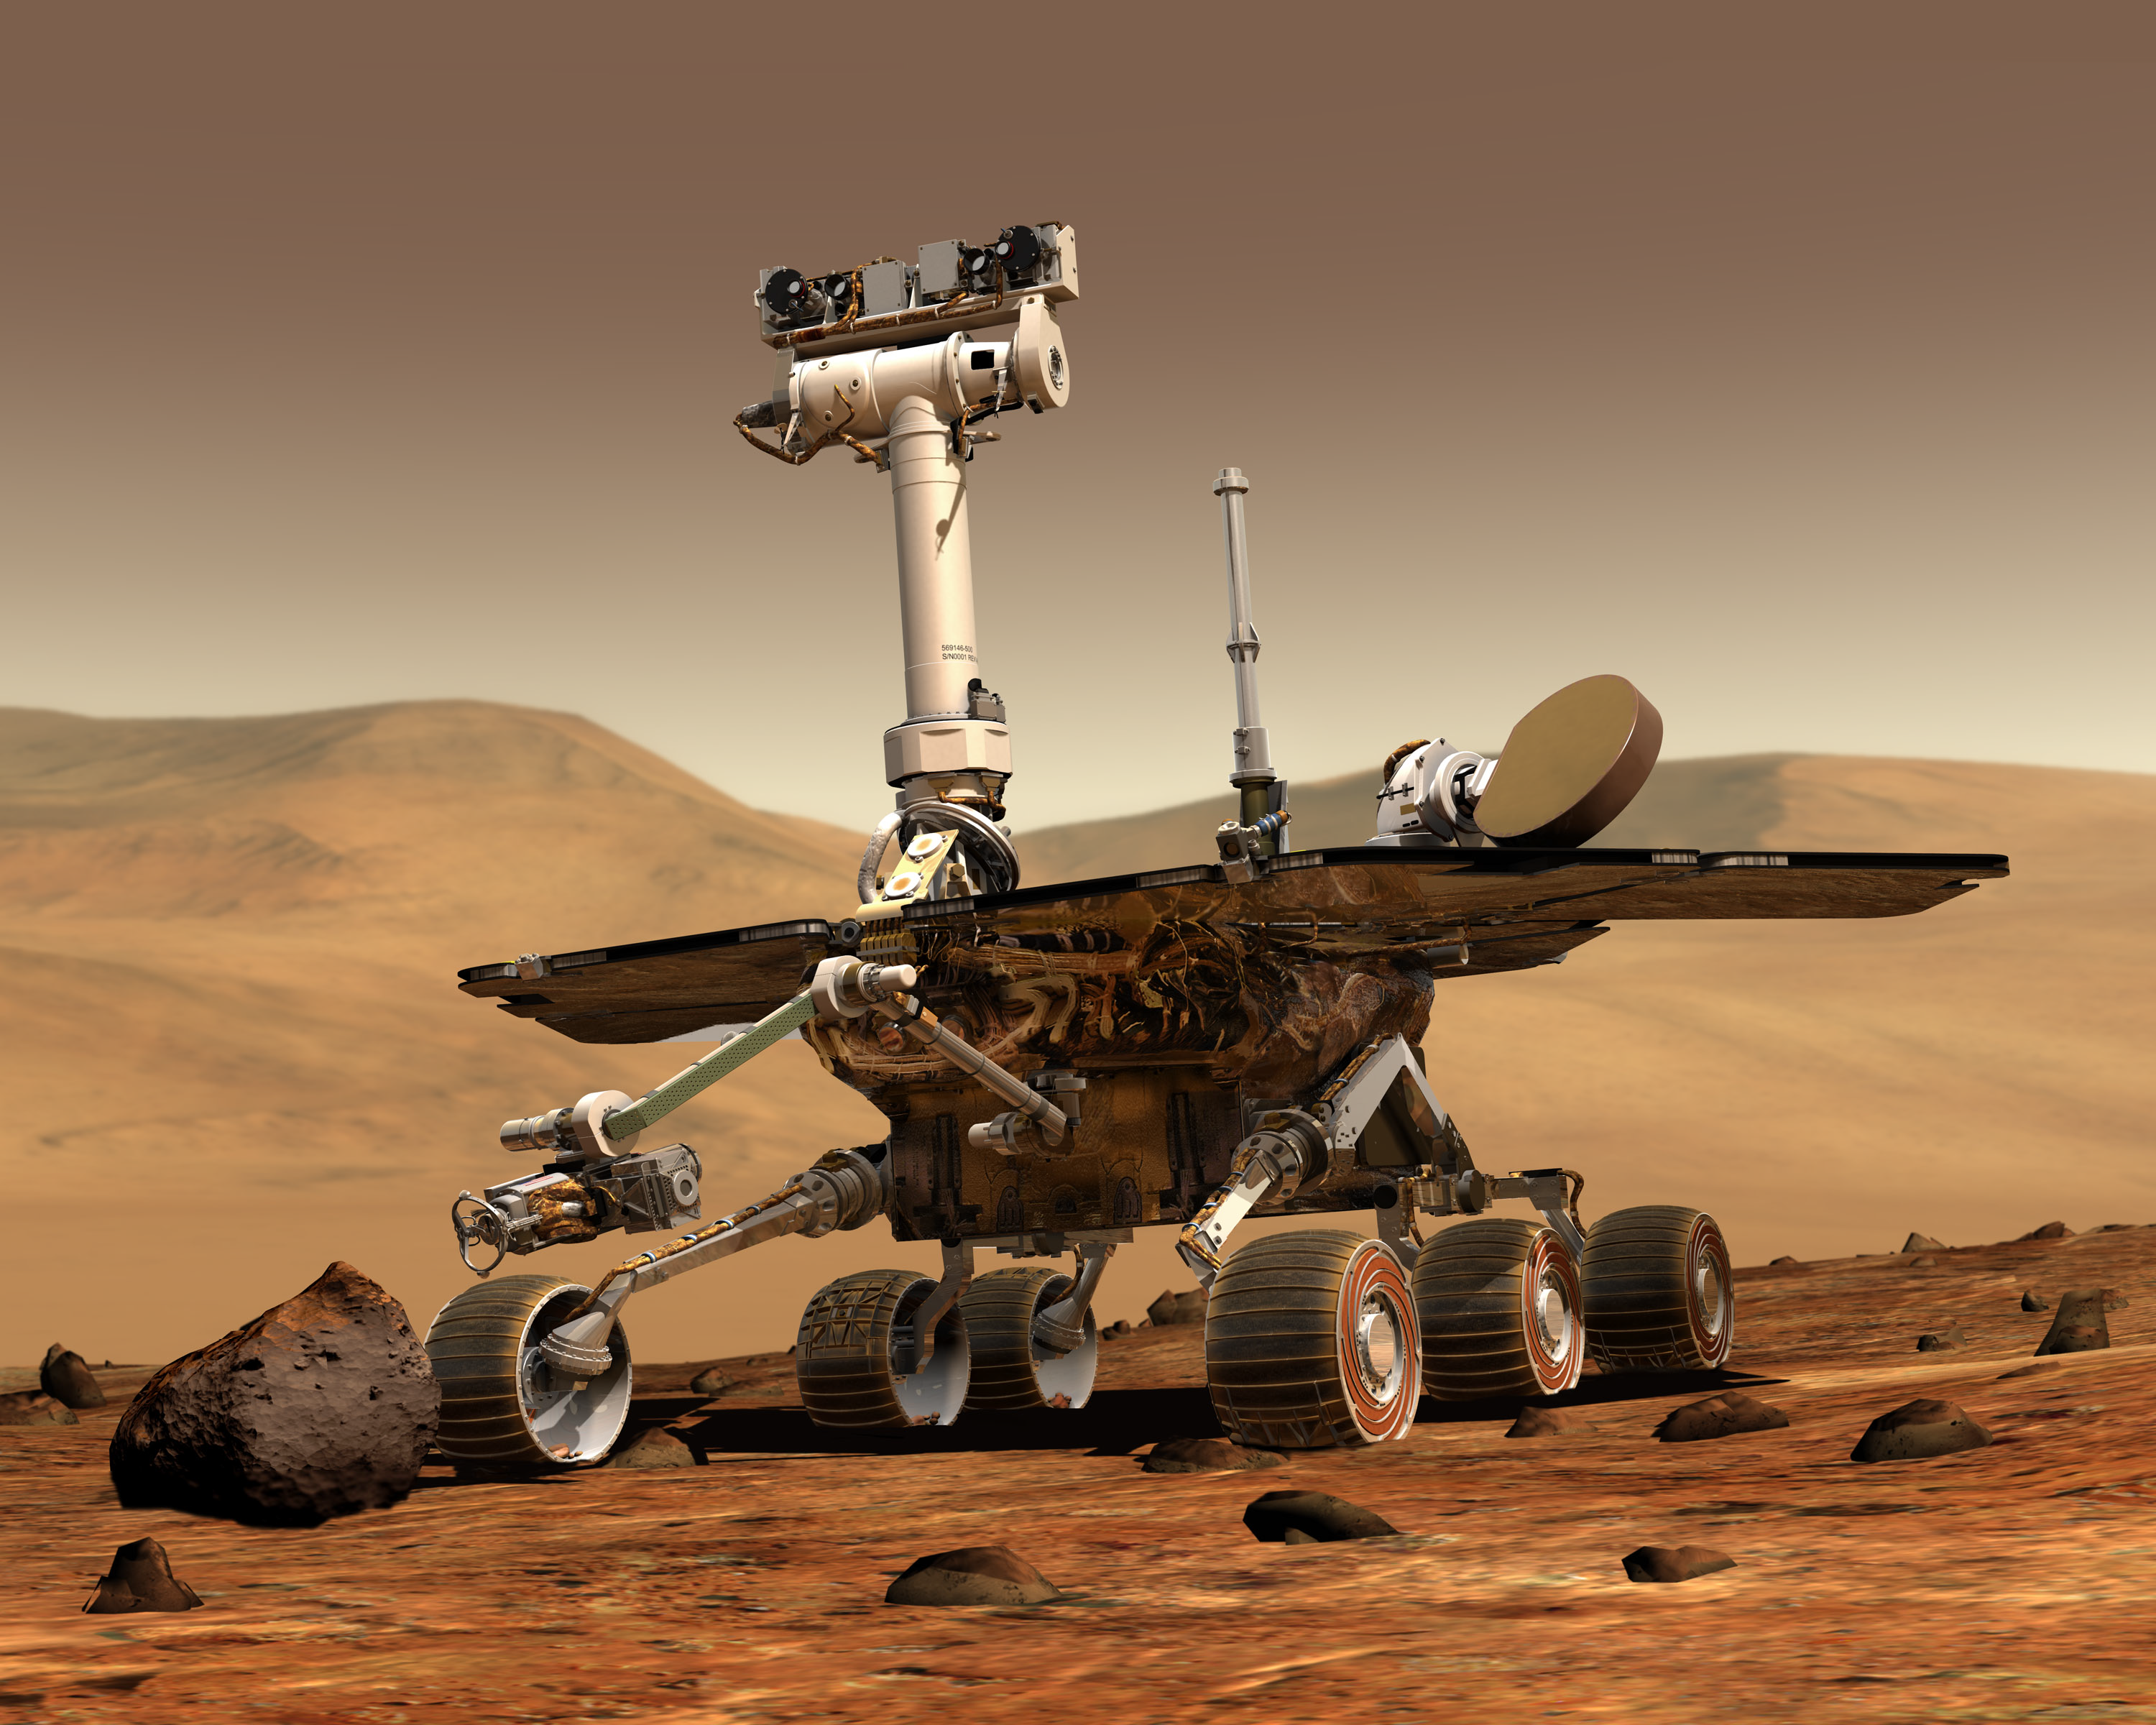
\includegraphics[width=3cm]{fig_01}\\
%\textit{}
}%figues de la page de garde

\def\xxtitreexo{Suite de Syracuse}
\def\xxsourceexo{}
\def\xxactivite{TP 01 -- Bonus \ifprof  -- Corrigé \else \fi}

%\iflivret
\input{\repRel/Style/pagegarde_TD}
%\else
%\pagestyle{empty}


%%%%%%%% PAGE DE GARDE COURS
\ifcours
% ==== BANDEAU DES TITRES ==== 
\begin{tikzpicture}[remember picture,overlay]
\node at (current page.north west)
{\begin{tikzpicture}[remember picture,overlay]
\node[anchor=north west,inner sep=0pt] at (0,0) {\includegraphics[width=\paperwidth]{\thechapterimage}};
\draw[anchor=west] (-2cm,-8cm) node [line width=2pt,rounded corners=15pt,draw=ocre,fill=white,fill opacity=0.6,inner sep=40pt]{\strut\makebox[22cm]{}};
\draw[anchor=west] (1cm,-8cm) node {\huge\sffamily\bfseries\color{black} %
\begin{minipage}{1cm}
\rotatebox{90}{\LARGE\sffamily\textsc{\color{ocre}\textbf{\xxnumpartie}}}
\end{minipage} \hfill
\begin{minipage}[c]{14cm}
\begin{titrepartie}
\begin{flushright}
\renewcommand{\baselinestretch}{1.1} 
\Large\sffamily\textsc{\textbf{\xxpartie}}
\renewcommand{\baselinestretch}{1} 
\end{flushright}
\end{titrepartie}
\end{minipage} \hfill
\begin{minipage}[c]{3.5cm}
{\large\sffamily\textsc{\textbf{\color{ocre} \discipline}}}
\end{minipage} 
 };
\end{tikzpicture}};
\end{tikzpicture}
% ==== FIN BANDEAU DES TITRES ==== 


% ==== ONGLET 
\begin{tikzpicture}[overlay]
\node[shape=rectangle, 
      rounded corners = .25 cm,
	  draw= ocre,
	  line width=2pt, 
	  fill = ocre!10,
	  minimum width  = 2.5cm,
	  minimum height = 3cm,] at (18.3cm,0) {};
\node at (17.7cm,0) {\rotatebox{90}{\textbf{\Large\color{ocre}{\classe}}}};
%{};
\end{tikzpicture}
% ==== FIN ONGLET 


\vspace{3.5cm}

\begin{tikzpicture}[remember picture,overlay]
\draw[anchor=west] (-2cm,-6cm) node {\huge\sffamily\bfseries\color{black} %
\begin{minipage}{2cm}
\begin{center}
\LARGE\sffamily\textsc{\color{ocre}\textbf{\xxactivite}}
\end{center}
\end{minipage} \hfill
\begin{minipage}[c]{15cm}
\begin{titrechapitre}
\renewcommand{\baselinestretch}{1.1} 
\Large\sffamily\textsc{\textbf{\xxnumchapitre}}

\Large\sffamily\textsc{\textbf{\xxchapitre}}
\vspace{.5cm}

\renewcommand{\baselinestretch}{1} 
\normalsize\normalfont
\xxcompetences
\end{titrechapitre}
\end{minipage}  };
\end{tikzpicture}
\vfill

\begin{flushright}
\begin{minipage}[c]{.3\linewidth}
\begin{center}
\xxfigures
\end{center}
\end{minipage}\hfill
\begin{minipage}[c]{.6\linewidth}
\startcontents
%\printcontents{}{1}{}
\printcontents{}{1}{}
\end{minipage}
\end{flushright}

\begin{tikzpicture}[remember picture,overlay]
\draw[anchor=west] (4.5cm,-.7cm) node {
\begin{minipage}[c]{.2\linewidth}
\begin{flushright}
\includegraphics[width=2cm]{logoCC}
\end{flushright}
\end{minipage}
\begin{minipage}[c]{.2\linewidth}
\textsl{\xxauteur} \\
\textsl{\classe}
\end{minipage}
 };
\end{tikzpicture}

\newpage
\pagestyle{fancy}

%\newpage
%\pagestyle{fancy}

\else
\fi
%% FIN PAGE DE GARDE DES COURS

%%%%%%%% PAGE DE GARDE TD
\iftd
%\begin{tikzpicture}[remember picture,overlay]
%\node at (current page.north west)
%{\begin{tikzpicture}[remember picture,overlay]
%\draw[anchor=west] (-2cm,-3.25cm) node [line width=2pt,rounded corners=15pt,draw=ocre,fill=white,fill opacity=0.6,inner sep=40pt]{\strut\makebox[22cm]{}};
%\draw[anchor=west] (1cm,-3.25cm) node {\huge\sffamily\bfseries\color{black} %
%\begin{minipage}{1cm}
%\rotatebox{90}{\LARGE\sffamily\textsc{\color{ocre}\textbf{\xxnumpartie}}}
%\end{minipage} \hfill
%\begin{minipage}[c]{13.5cm}
%\begin{titrepartie}
%\begin{flushright}
%\renewcommand{\baselinestretch}{1.1} 
%\Large\sffamily\textsc{\textbf{\xxpartie}}
%\renewcommand{\baselinestretch}{1} 
%\end{flushright}
%\end{titrepartie}
%\end{minipage} \hfill
%\begin{minipage}[c]{3.5cm}
%{\large\sffamily\textsc{\textbf{\color{ocre} \discipline}}}
%\end{minipage} 
% };
%\end{tikzpicture}};
%\end{tikzpicture}

%%%%%%%%%% PAGE DE GARDE TD %%%%%%%%%%%%%%%
%\begin{tikzpicture}[overlay]
%\node[shape=rectangle, 
%      rounded corners = .25 cm,
%	  draw= ocre,
%	  line width=2pt, 
%	  fill = ocre!10,
%	  minimum width  = 2.5cm,
%	  minimum height = 2.5cm,] at (18.5cm,0) {};
%\node at (17.7cm,0) {\rotatebox{90}{\textbf{\Large\color{ocre}{\classe}}}};
%%{};
%\end{tikzpicture}

% PARTIE ET CHAPITRE
%\begin{tikzpicture}[remember picture,overlay]
%\draw[anchor=west] (-1cm,-2.1cm) node {\large\sffamily\bfseries\color{black} %
%\begin{minipage}[c]{15cm}
%\begin{flushleft}
%\xxnumchapitre \\
%\xxchapitre
%\end{flushleft}
%\end{minipage}  };
%\end{tikzpicture}

% BANDEAU EXO
\iflivret % SI LIVRET
\begin{tikzpicture}[remember picture,overlay]
\draw[anchor=west] (-2cm,-3.3cm) node {\huge\sffamily\bfseries\color{black} %
\begin{minipage}{5cm}
\begin{center}
\LARGE\sffamily\color{ocre}\textbf{\textsc{\xxactivite}}

\begin{center}
\xxfigures
\end{center}

\end{center}
\end{minipage} \hfill
\begin{minipage}[c]{12cm}
\begin{titrechapitre}
\renewcommand{\baselinestretch}{1.1} 
\large\sffamily\textbf{\textsc{\xxtitreexo}}

\small\sffamily{\textbf{\textit{\color{black!70}\xxsourceexo}}}
\vspace{.5cm}

\renewcommand{\baselinestretch}{1} 
\normalsize\normalfont
\xxcompetences
\end{titrechapitre}
\end{minipage}};
\end{tikzpicture}
\else % ELSE NOT LIVRET
\begin{tikzpicture}[remember picture,overlay]
\draw[anchor=west] (-2cm,-4.5cm) node {\huge\sffamily\bfseries\color{black} %
\begin{minipage}{5cm}
\begin{center}
\LARGE\sffamily\color{ocre}\textbf{\textsc{\xxactivite}}

\begin{center}
\xxfigures
\end{center}

\end{center}
\end{minipage} \hfill
\begin{minipage}[c]{12cm}
\begin{titrechapitre}
\renewcommand{\baselinestretch}{1.1} 
\large\sffamily\textbf{\textsc{\xxtitreexo}}

\small\sffamily{\textbf{\textit{\color{black!70}\xxsourceexo}}}
\vspace{.5cm}

\renewcommand{\baselinestretch}{1} 
\normalsize\normalfont
\xxcompetences
\end{titrechapitre}
\end{minipage}};
\end{tikzpicture}

\fi

\else   % FIN IF TD
\fi


%%%%%%%% PAGE DE GARDE FICHE
\iffiche
\begin{tikzpicture}[remember picture,overlay]
\node at (current page.north west)
{\begin{tikzpicture}[remember picture,overlay]
\draw[anchor=west] (-2cm,-2.25cm) node [line width=2pt,rounded corners=15pt,draw=ocre,fill=white,fill opacity=0.6,inner sep=40pt]{\strut\makebox[22cm]{}};
\draw[anchor=west] (1cm,-2.25cm) node {\huge\sffamily\bfseries\color{black} %
\begin{minipage}{1cm}
\rotatebox{90}{\LARGE\sffamily\textsc{\color{ocre}\textbf{\xxnumpartie}}}
\end{minipage} \hfill
\begin{minipage}[c]{14cm}
\begin{titrepartie}
\begin{flushright}
\renewcommand{\baselinestretch}{1.1} 
\large\sffamily\textsc{\textbf{\xxpartie} \\} 

\vspace{.2cm}

\normalsize\sffamily\textsc{\textbf{\xxnumchapitre -- \xxchapitre}}
\renewcommand{\baselinestretch}{1} 
\end{flushright}
\end{titrepartie}
\end{minipage} \hfill
\begin{minipage}[c]{3.5cm}
{\large\sffamily\textsc{\textbf{\color{ocre} \discipline}}}
\end{minipage} 
 };
\end{tikzpicture}};
\end{tikzpicture}

\iflivret
\begin{tikzpicture}[overlay]
\node[shape=rectangle, 
      rounded corners = .25 cm,
	  draw= ocre,
	  line width=2pt, 
	  fill = ocre!10,
	  minimum width  = 2.5cm,
	  minimum height = 2.5cm,] at (18.5cm,1.1cm) {};
\node at (17.9cm,1.1cm) {\rotatebox{90}{\textsf{\textbf{\large\color{ocre}{\classe}}}}};
%{};
\end{tikzpicture}
\else
\begin{tikzpicture}[overlay]
\node[shape=rectangle, 
      rounded corners = .25 cm,
	  draw= ocre,
	  line width=2pt, 
	  fill = ocre!10,
	  minimum width  = 2.5cm,
%	  minimum height = 2.5cm,] at (18.5cm,1.1cm) {};
	  minimum height = 2.5cm,] at (18.6cm,1cm) {};
\node at (18cm,1cm) {\rotatebox{90}{\textsf{\textbf{\large\color{ocre}{\classe}}}}};
%{};
\end{tikzpicture}

\fi

\else
\fi



%\fi

\setlength{\columnseprule}{.1pt}

\pagestyle{fancy}
\thispagestyle{plain}

\vspace{4.5cm}

\def\columnseprulecolor{\color{bleuxp}}
\setlength{\columnseprule}{0.4pt} 

%%%%%%%%%%%%%%%%%%%%%%%




\ifprof
\vspace{1cm}
\else
\begin{multicols}{2}
\fi

\exer{La conjecture de Syracuse}
\setcounter{numques}{0}~\\

\begin{flushright}
\textit{D'après Jean-Pierre Becirspahic, \url{https://info-llg.fr/}}
\end{flushright}
\begin{obj} ~\\
\begin{itemize}
\item ...
\end{itemize}
\end{obj}


On doit cette conjecture au mathématicien allemand Lothar Collatz qui, en 1937, proposa à la communauté mathématique
le problème suivant : << on part d’un nombre entier strictement positif ; s’il est pair on le divise par 2, s’il est impair on le multiplie par 3 et on ajoute 1. On réitère ensuite cette opération.>>

Par exemple, à partir de 14 on construit la suite de nombres :
$$14 ,7 ,22 ,11 ,34, 17, 52, 26, 13, 40, 20, 10, 5, 16, 8, 4, 2, 1, 4, 2 ...$$
Après que le nombre 1 ait été atteint, la suite des valeurs (1, 4, 2, 1, 4, 2 ...) se répète indéfiniment en un cycle de
longueur 3.

La conjecture de Syracuse\footnote{Du nom de l’université américaine qui a popularisé ce problème.} est l’hypothèse mathématique selon laquelle n’importe quel entier de départ conduit à la valeur 1 au bout d’un certain temps.

Nous allons expérimenter cette conjecture en programmant l’évolution de la suite $\left(u_n\right)_{n\in \mathbb{N}}$ définie par les relations :
$$
u_0=c \;\text{et} \; \forall n\geq 1, u_{n+1}=\left\{
\begin{array}{ll} 
\dfrac{u_n}{2} & \text{si }u_n \text{ est pair}\\
3 u_n + 1  & \text{si }u_n \text{ est impair}
\end{array} \right. .
$$

\subsection*{Temps de vol et altitude maximale}
Le temps de vol d’un entier $c$ et le plus petit entier $n$ (en admettant qu’il existe) pour lequel $u_n = 1$. Par exemple, le temps de vol pour $c = 14$ est égal à 17.

\question{Définir une fonction nommée \texttt{tempsdevol} prenant un paramètre entier \texttt{c} et retournant le plus petit entier $n$ pour lequel $u_n = 1$.}

De manière tout aussi imagée, on appelle altitude maximale de c la valeur maximale de la suite $\left(u_n\right)_{n\in \mathbb{N}}$. Par exemple, l’altitude maximale de $c = 14$ est égale à 52.

\question{Modifier votre algorithme pour définir une fonction nommée \texttt{altitude} qui calcule cette fois-ci l’altitude maximale pour un entier $c$ donné en paramètre.}

\subsection*{Vérification expérimentale de la conjecture}

On désire désormais vérifier la validité de la conjecture pour toute valeur $c \leq 1\,000\, 000$. Une première solution consisterait à calculer le temps de vol pour toutes ces valeurs, mais ce calcul est long et il y a mieux à faire en observant que si la conjecture a déjà été vérifiée pour toute valeur $c'<c$, il suffit qu’il existe un rang $n$ pour lequel $u_n < c$ pour être certain que la conjecture sera aussi vérifiée au rang $c$.


On appelle temps d’arrêt (ou encore temps de vol en altitude) le premier entier $n$ (s’il existe) pour lequel $u_n < c$.

\question{ Écrire une fonction \texttt{tempsdarret} prenant un paramètre entier $c$ et retournant le temps d’arrêt de la suite de Syracuse correspondante.}

Nous souhaitons maintenant mesurer le temps nécessaire pour vérifier la conjecture jusqu’à un paramètre entier $m$. Pour cela, nous allons utiliser la fonction \texttt{time} du module time du même nom, sans argument, qui retourne le temps en secondes depuis une date de référence (qui dépend du système).

\question{À l’aide de cette fonction écrire une fonction \texttt{verification} qui prend en argument un paramètre entier $m$ et retourne le temps nécessaire pour vérifier que toutes les valeurs $c\in \llbracket 2,m \rrbracket$  ont bien un temps d’arrêt fini.
Quelle durée d’exécution obtient-t-on pour $ m = 1\,000\,000$ ?}

\question{Quel est le temps d’arrêt d’un entier pair ? et d’un entier de la forme $c = 4n + 1$ ? En déduire qu’on peut restreindre la
recherche aux entiers de la forme $4n+ 3$, et modifier en conséquence la fonction précédente. Combien de temps gagne-t-on
par rapport à la version précédente pour $m = 1\,000\,000$ ?
Vérifier ensuite la conjecture pour $m = 10\,000\,000$.
}

\subsection*{Records}
\question{Déterminer l’altitude maximale que l’on peut atteindre lorsque $c \in \llbracket 1,1\,000\,000\rrbracket$, ainsi que la valeur minimale de $c$ permettant d’obtenir cette altitude.}

\question{Déterminer le temps de vol en altitude (autrement dit le temps d’arrêt) de durée maximale lorsque $c \in \llbracket 1,1\,000\,000\rrbracket$ 
ainsi que la valeur de $c$ correspondante.}


\question{On appelle vol en altitude de durée record un vol dont tous les temps d’arrêt de rangs inférieurs sont plus courts. Par exemple, le vol réalisé pour $c = 7$ est un vol en altitude de durée record (égale à 11) car tous les vols débutant
par $c = 1,2,3,4,5,6$ ont des temps d’arrêt de durées inférieures à 11. Déterminez tous les vols en altitude de durée record
pour $c \leq 1\,000\,000$.}

\subsection*{Affichage du vol}

Pour obtenir des graphes, on utilise la fonction plot qui appartient à un module appelé
\texttt{matplotlib.pyplot} et dédié au tracé de graphes. Vous allez donc commencer par importer celui-ci à l’aide de la
commande :
\texttt{import matplotlib.pyplot as plt}
Désormais toutes les fonctions de ce module vous sont accessibles à condition de les préfixer par \texttt{plt}. Nous découvrirons
progressivement les nombreuses possibilités qu’offre ce module, mais aujourd’hui nous n’aurons besoin que de deux
fonctions : \texttt{plt.plot} et \texttt{plt.show}.
Sous sa forme la plus simple, la fonction \texttt{plt.plot} n’exige qu’une liste en paramètre : \texttt{plt.plot([a0, a1, ..., an])}
crée un graphe constitué d’une ligne brisée reliant les points de coordonnées $(k,a_k
)$ pour $k \in  \llbracket 0,n \rrbracket$.
En Python, une liste est encadrée par des crochets et ses éléments séparés par une virgule. Nous étudierons les listes plus
tard dans le cours ; pour l’instant nous n’aurons besoin que du résultat suivant : si \texttt{lst} est une liste, on ajoute un élément
\texttt{x} à celle-ci à l’aide de la commande : \texttt{lst.append(x)}.
Une fois votre graphe créé par la fonction \texttt{plt.plot}, il reste à le faire apparaître dans une fenêtre annexe à l’aide de
l’instruction \texttt{plt.show()}.

\question{Définir une fonction nommée graphique qui prend un entier $c$ en paramètre et qui construit le graphe de
la suite $\left(u_n\right)_{n\in \mathbb{N}}$ durant son temps de vol.}



\ifprof
\else
\end{multicols}
\fi

